\subsection{Transfer grid velocities to particles}

As we could see in the previous section, going from particle velocities to grid can be a bit tricky when working with a MAC grid. Luckily, going from grid velocities to particle velocities is a lot easier. For every particle, we will use bilinear interpolation to get the horizontal and vertical velocities.

\begin{figure}[ht!]
\centering
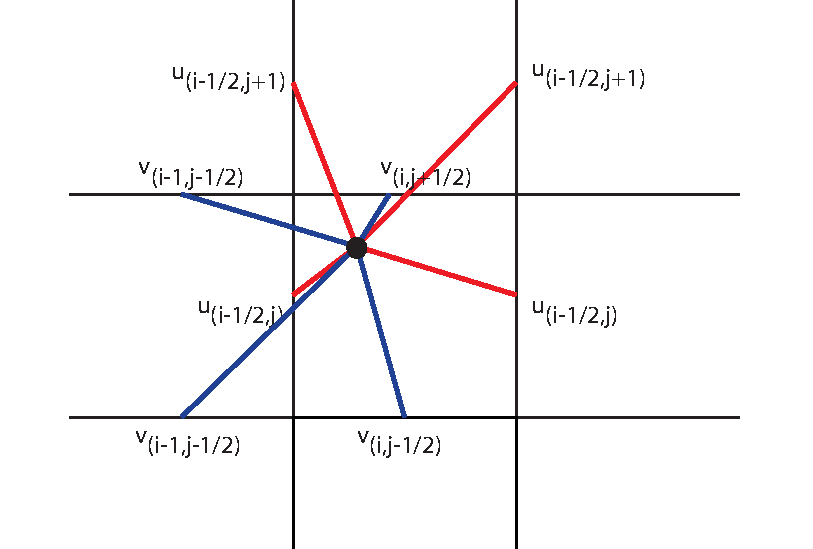
\includegraphics[width=80mm]{img/splat.pdf}
\caption{The particle velocity $\vec{u}_p$ is bilineary interpolated between neighboring velocities in the MAC grid.}
\label{onedge}
\end{figure}
\noindent
The FLIP part of our hybrid particle-grid approach is how we update the particle velocities. If we only update the particles with the velocities that the pressure solving step gives us, it is called \emph{Particle in Cell}, PIC, which is an older approach. Zhou and Bridson \cite{chu} are in their FLIP paper, before solving the pressure equations, saving the old divergence-free velocity field and then updating the particles with the change of velocity instead of only the new velocity.

\begin{equation}
\Delta \vec{u} = \vec{u}^{n+1} - \vec{u}^n
\end{equation}
\noindent
FLIP alone can cause a lot of noise because of the large particle count. The FLIP paper recommends linear interpolation between FLIP and PIC for best result. The formula for updated particle velocities can be expressed as:

\begin{equation}
\vec{u}_p = \alpha \cdot bilerp(\vec{u}^{n+1}, \vec{x}_p) + (1-\alpha) \cdot bilerp(\Delta \vec{u},\vec{x}_p)
\label{flipeq}
\end{equation}

where $\alpha$ is a number between $0$ and $1$. If one, it is only PIC and zero is pure FLIP. Values closer to one gives a more stable look but to the cost of more numerical dissipation which cancels out a lot of the interesting high frequency motion.
